\documentclass{beamer}
%\documentclass[handout]{beamer}

% language settings
%\usepackage{fontspec, polyglossia}
%\setdefaultlanguage{magyar}

% common packages
\usepackage{amsmath, multimedia, hyperref, color, multirow}
%\usepackage{graphicx}

% TikZ
\usepackage{tikz}
%\usetikzlibrary{arrows.meta, decorations.pathmorphing, decorations.pathreplacing, shapes.geometric,mindmap}
%\usetikzlibrary{shapes.geometric,fadings,bayesnet}

% beamer styles
\mode<presentation>{
\usetheme{Boadilla}
%\usetheme{Antibes}
%\usecolortheme{beaver}
%\usecolortheme{seahorse}
%\usefonttheme{structureitalicserif}
\setbeamercovered{transparent}
}
\setbeamertemplate{blocks}[rounded][shadow=true]
\AtBeginSubsection[]{
  \begin{frame}<beamer>{Contents}
    \tableofcontents[currentsection,currentsubsection]
  \end{frame}
}
%\useoutertheme[]{tree}

% title, etc
\title{The ``Imprinting Manuscript''}
\subtitle{Normal Expression Bias of Imprinted Genes in Schizophrenics}
\author{Attila Gulyas-Kovacs}
\date{Chess lab meeting 12/12/17}

\begin{document}

\maketitle

\begin{frame}[label=cmc]{The CommonMind data}
\includegraphics[width=1.0\textwidth]{figures/by-me/commonmind-rna-seq/commonmind-rna-seq.pdf}
\end{frame}

\begin{frame}
\begin{itemize}
\item questions
\begin{enumerate}
\item schizophrenia and imprinting (15q11-q13 microduplications)
\item imprinted genes in adult human DLPFC
\item determinants of imprinting (age, ancestry, gender)
\end{enumerate}
\item key studies
\begin{enumerate}
\item Fromer et al 2016 Nat Neurosci
\item Gregg et al 2010 Science
\item Baran et al 2015 Genome Res
\item Perez et al 2015 eLife 
\end{enumerate}
\end{itemize}
\end{frame}

\begin{frame}{\emph{Read count ratio} gauges \emph{allelic bias} and thus \emph{imprinting}}
\includegraphics[width=1.0\textwidth]{figures/by-me/commonmind-rna-seq-ms/commonmind-rna-seq-ms.pdf}
\end{frame}

\begin{frame}{Ranking genes based on variation across individuals}
\begin{center}
\includegraphics[height=0.85\textheight]{figures/2016-07-19-genome-wide-S/complex-plot-1.png}
\end{center}
\end{frame}

\begin{frame}{Gene score and previous imprinted gene clusters}
\begin{center}
\includegraphics[height=0.85\textheight]{figures/2016-08-08-imprinted-gene-clusters/score-genomic-location-1.png}
\end{center}
\end{frame}

\begin{frame}{Establishing imprinting status in the human DLPFC}
\begin{columns}[t]
\begin{column}{0.5\textwidth}
\begin{itemize}
\item prior expectation: near cluster
\item alternative causes of high read count ratio
\begin{enumerate}
\item mapping bias
\item eQTL
\end{enumerate}
\end{itemize}
\end{column}
\begin{column}{0.5\textwidth}

\includegraphics[height=0.85\textheight]{figures/2016-08-01-ifats-filters/top-ranking-genes-1.pdf}
\end{column}
\end{columns}
\end{frame}

\begin{frame}{Including 3 slightly lower scoring genes}
\begin{center}
\includegraphics[height=0.85\textheight]{figures/2016-08-01-ifats-filters/known-genes-1.pdf}
\end{center}
\end{frame}

\begin{frame}{Explaining variation with psychiatric diagnosis, Dx}
{The simple but ``confounded'' approach}
\begin{center}
\includegraphics[height=0.85\textheight]{figures/2016-11-01-plotting-distribution-of-s/S-Dx-strip-1.pdf}
\end{center}
\end{frame}

\begin{frame}{More information with more explanatory variables}
\begin{table}[H]
\begin{center}
\begin{tabular}{r|l}
explanatory variable & levels\\
\hline
Age &  \\
Institution & [MSSM], Penn, Pitt\\
Gender & [Female], Male\\
PMI & \\
Dx & [Control], SCZ, AFF \\
RIN &  \\
RNA\_batch & [A], B, C, D, E, F, G, H, 0\\
Ancestry.1 & \\
\vdots & \\
Ancestry.5 &  \\
\end{tabular}
\end{center}
\end{table}
\end{frame}

\begin{frame}{Dependencies: the source of confounding}
\begin{center}
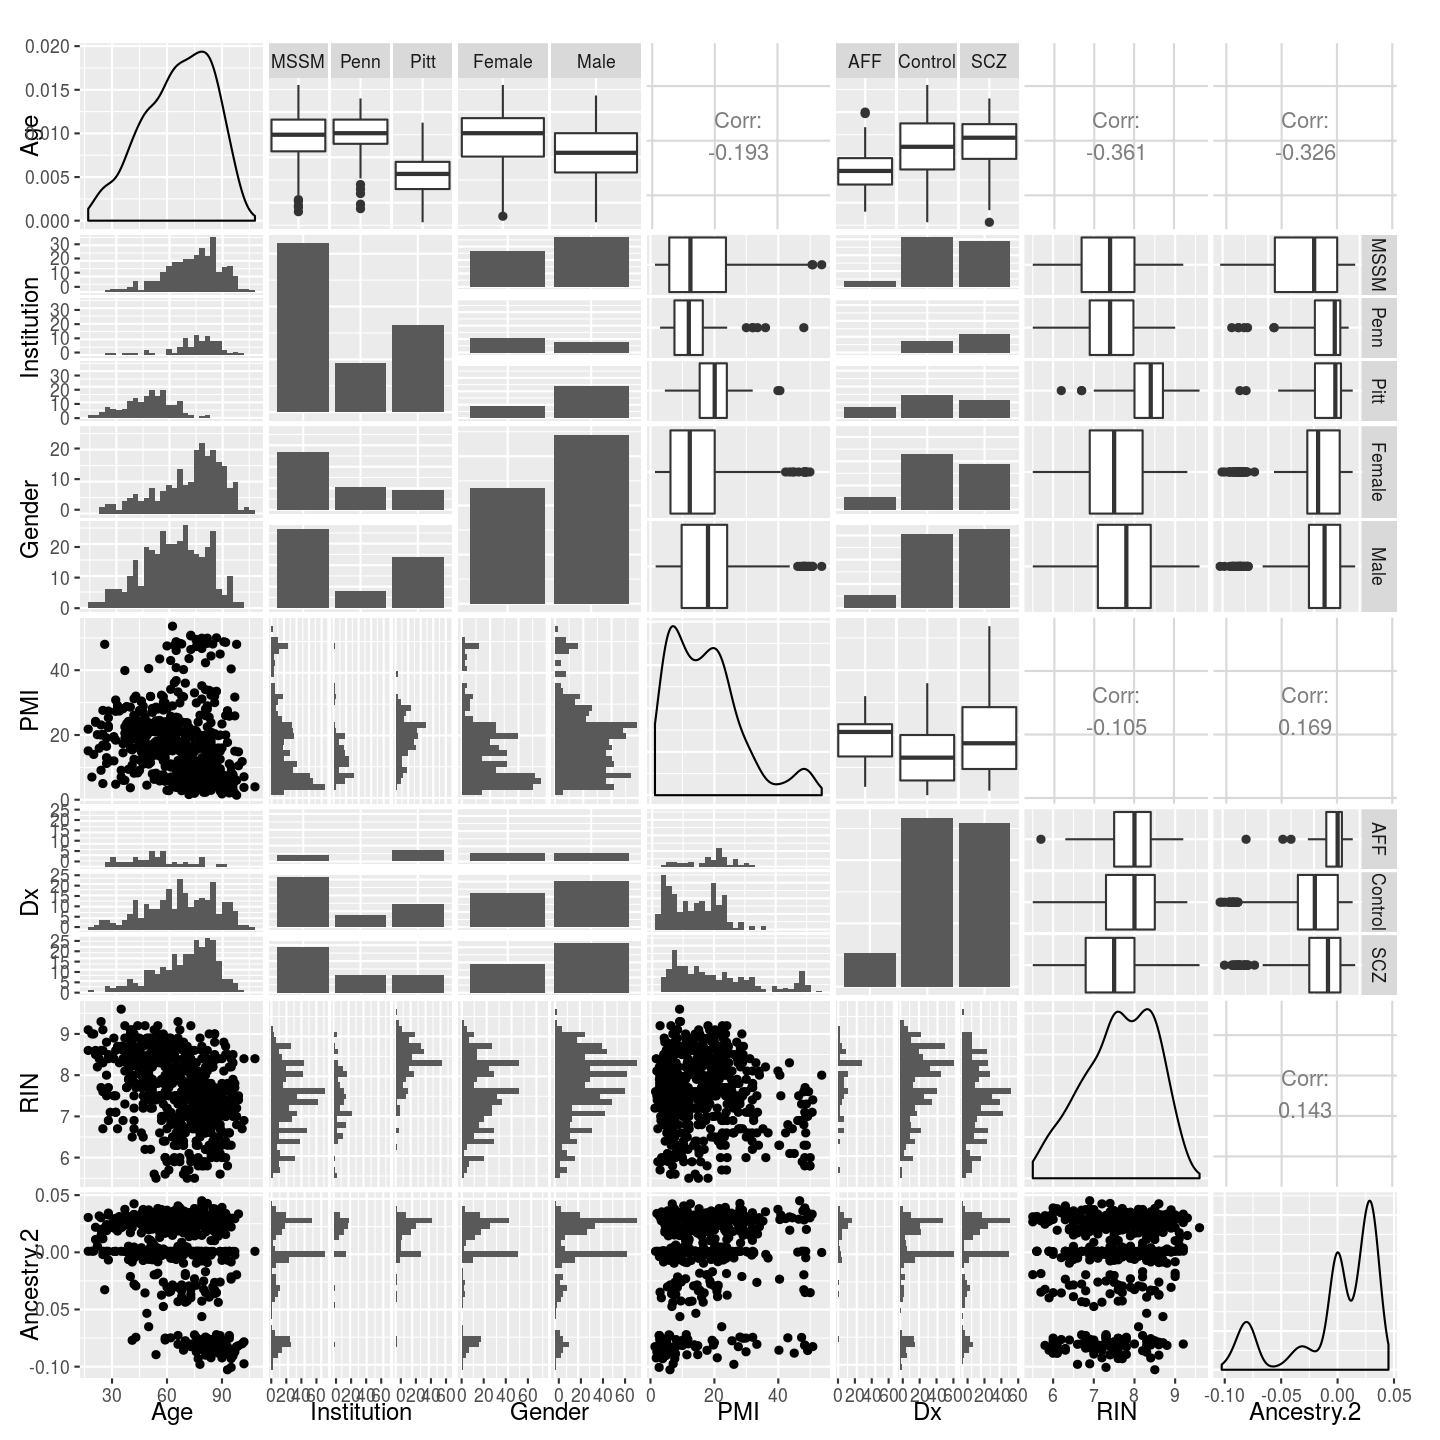
\includegraphics[height=0.85\textheight]{figures/2016-06-26-trellis-display-of-data/evar-scatterplot-matrix-2.png}
\end{center}
\end{frame}

\begin{frame}<1-2>[label=models]{Several regression models of read count ratio \(Y_g\)}
Quantities
\begin{itemize}
\item<2-> observed variables
\begin{itemize}
\item<2-> \(Y_{g} = S_g\): response \(=\) read count ratio for gene \(g\)
\item<2-> \(Y_g = Q_{g}\) (or \(Y_g = R_g\)): response \(=\) transformed read count ratio
\item<3-> \(X_{j}\): the \(j\)-th column of design matrix \(X\)
\end{itemize}
\item<3-> model parameters
\begin{itemize}
\item<3-> \(\beta_{jg}\) (or \(b_{jg}\)): regression coefficient for \(Y_g\) and \(X_{j}\)
\item<3-> \(\sigma_g\) (or \(m_{ig}\)): parameters for noise 
\end{itemize}
\end{itemize}
\vfill
Properties
\begin{itemize}
\item<4-> given \(g\), the structure of dependencies among \(Y_g, X_1,...,X_p\)
\item<5-> parametric family (normal or logistic)
\begin{itemize}
\item<5-> link function
\item<5-> noise distribution 
\end{itemize}
\end{itemize} 
\end{frame}

\begin{frame}[label=untransformed]{Untransformed read count ratio \(S_g\)}
\begin{center}
\includegraphics[height=0.85\textheight]{figures/2016-11-01-plotting-distribution-of-s/S-Dx-age-1.pdf}
\end{center}
\end{frame}

\begin{frame}[label=transformed]{Transformed read count ratio \(Q_g\)}
\begin{center}
\includegraphics[height=0.85\textheight]{figures/2016-11-01-plotting-distribution-of-s/Q-Dx-age-1.pdf}
\end{center}
\end{frame}

\againframe<2-4>{models}

\begin{frame}{Three classes of dependency structure}
\begin{columns}[t]
\begin{column}{0.33\textwidth}
\emph{fixed I}

\includegraphics[scale=0.8]{figures/by-me/monoall-dependencies-2/obs-simple-general/obs-simple-general}
\end{column}

\begin{column}{0.33\textwidth}
\emph{fixed II}

\includegraphics[scale=0.8]{figures/by-me/monoall-dependencies-2/obs-simple-general-gene-aspec/obs-simple-general-gene-aspec}
\end{column}
\begin{column}{0.33\textwidth}
\emph{mixed}

\includegraphics[scale=0.8]{figures/by-me/monoall-dependencies-2/mixed/mixed}
\end{column}
\end{columns}
\vfill
\begin{itemize}
\item fixed I: too complex \(\Rightarrow\) low power
\item fixed II: too simplistic \(\Rightarrow\) bias
\item mixed: powerful middle ground---even with interactions
\end{itemize}
\end{frame}

\againframe<4->{models}

\begin{frame}{Parametric families}
\begin{table}[H]
\begin{center}
\begin{tabular}{ccc}
%\multicolumn{2}{c}{\replaced{link function and error distribution}{regression models}} \\
model family & abbrev. & response var.~\\
\hline
\emph{u}nweighted \emph{n}ormal \emph{l}inear & unlm  & \(S, Q,\) or \(R\) \\
\emph{w}eighted \emph{n}ormal \emph{l}inear & wnlm  & \(S, Q,\) or \(R\) \\
\emph{logi}stic & logi & \(S\) \\
\emph{logi}stic, \(\frac{1}{2}\times\) down-scaled link fun.~& logi2 & \(S\) \\
\end{tabular}
\end{center}
\end{table}
\end{frame}

\begin{frame}{Fit of fixed I models for PEG3}
\includegraphics[width=0.35\textwidth]{figures/2016-08-23-glm-sampling-distributions/PEG3-1.png}
\includegraphics[width=0.35\textwidth]{figures/2016-09-23-model-checking/qqnorm-PEG3-1.pdf}

\includegraphics[width=0.35\textwidth]{figures/2016-09-23-model-checking/homoscedas-PEG3-1.pdf}
\includegraphics[width=0.35\textwidth]{figures/2016-09-23-model-checking/influence-PEG3-1.pdf}
\end{frame}

\begin{frame}{Fit of fixed I models for KCNK9}
\includegraphics[width=0.35\textwidth]{figures/2016-08-23-glm-sampling-distributions/KCNK9-1.png}
\includegraphics[width=0.35\textwidth]{figures/2016-09-23-model-checking/qqnorm-KCNK9-1.pdf}

\includegraphics[width=0.35\textwidth]{figures/2016-09-23-model-checking/homoscedas-KCNK9-1.pdf}
\includegraphics[width=0.35\textwidth]{figures/2016-09-23-model-checking/influence-KCNK9-1.pdf}
\end{frame}

\begin{frame}{Fit of mixed models (all genes jointly)}
\begin{center}
\includegraphics[width=0.45\textwidth]{figures/2017-03-08-model-checking/qqplot-families-M3-1.pdf}
\includegraphics[width=0.45\textwidth]{figures/2017-03-08-model-checking/scedasticity-families-M3-1.pdf}
\end{center}
\end{frame}

\begin{frame}{Regression coefficients}
\begin{columns}[t]
\begin{column}{0.5\textwidth}

\includegraphics[height=0.85\textheight]{figures/2016-06-22-extending-anova/reg-coef-unlm-Q-ms-1.pdf}
\end{column}

\begin{column}{0.5\textwidth}

\includegraphics[height=0.85\textheight]{figures/2017-07-31-mixed-model-coefs/ranef-gender-gender-gene-m5-all-panels-1.pdf}
\end{column}
\end{columns}
\end{frame}

\begin{frame}{Testing independence of read count ratio}
{Based on unlmQ mixed model}
\tiny
\begin{table}[H]
\begin{center}
\begin{tabular}{rlrc}
predictor term                              & interpretation&   \(\Delta\)AIC &        p-value \\
\hline
\((1\,|\,\mathrm{Gene})\)                   & variability among genes & \(-126.8\)  & \(8.5\times 10^{-28}\) \\
\((1\,|\,\mathrm{Dx})\)                     & variability among Control, SCZ, AFF & \(2.0\)  & \(1.0\)  \\
\((1\,|\,\mathrm{Dx}:\mathrm{Gene})\)       & Gene specific variability among Ctrl, SCZ, AFF & \(0.4\) &  \(0.21\) \\
\(\mathrm{Age}\)                            & effect of Age & \(1.3\)   & \(0.39\) \\
\((\mathrm{Age}\,|\,\mathrm{Gene})\)        & Gene specific effect of Age & \(-18.9\)  & \(2.5\times 10^{-5}\)  \\
\(\mathrm{Ancestry.1}\)                     & effect of Ancestry.1 & \(0.6\)  & \(0.24\) \\
\((\mathrm{Ancestry.1}\,|\,\mathrm{Gene})\) & Gene specific effect of Ancestry.1 & \(-71.2\)   & \(4.6\times 10^{-16}\) \\
\(\mathrm{Ancestry.3}\)                     & effect of Ancestry.3 & \(1.6\)  & \(0.54\) \\
\((\mathrm{Ancestry.3}\,|\,\mathrm{Gene})\) & Gene specific effect of Ancestry.3 & \(-17.9\)   & \(3.8\times 10^{-5}\) \\
\((1\,|\,\mathrm{Gender})\)                 & difference between Male and Female & \(2.0\)  & \(1.0\)  \\
\((1\,|\,\mathrm{Gender}:\mathrm{Gene})\)   & Gene specific difference between M and F & \(-5.7\) &  \(5.5\times 10^{-3}\) \\
\end{tabular}
\end{center}
\end{table}
\end{frame}

\againframe{untransformed}

\begin{frame}{Summary}
\begin{enumerate}
\item CommonMind RNA-seq read count ratio gauging allelic bias
\item<2-> \(\approx\) 30 imprinted genes in human DLPFC
\begin{itemize}
\item in agreement with more recent estimates
\end{itemize}
\item<3-> normal allelic bias of imprinted genes in schizophrenics
\begin{itemize}
\item subtle effect + noise and bias?
\item complex genetic architecture
\end{itemize}
\item<4-> gene-specific effect of ancestry, gender, and age 
\begin{itemize}
\item aging: ``imprinting and the social brain''
\item ``DNA methylation age'' 
\end{itemize}
\end{enumerate}
\end{frame}

\end{document}



\begin{columns}[t]
\begin{column}{0.5\textwidth}

\end{column}

\begin{column}{0.5\textwidth}

\end{column}
\end{columns}
